\cotefile{70}
\scanpage{111}
% archive sheet number: 110
Icosaèdre géométrique et représentations du groupe $\Gamma$

Soit $\Pi=(S,A,F;r)$ l'icosaèdre combinatoire-type, épinglé par le \unsure{repère|racine} $r=\deleted{\unsure{(s_0)}}(s_0,\unsure{\mathrm{ar}|\mathrm{dr}}(s_0,s_1),\unsure{\mathrm{fl}}(s_0,s_1,s_2))$, $\Gamma$ son \unsure{gpe|groupe} des autom. Une \uline{représentation}\inserted{ou \uline{réalisation}} \uline{affine} \deleted{\unsure{régulière}} de $\Pi$ dans un \deleted{\unsure{espace}} \inserted{fibré} affine $E$ (sur schéma $S$) de dim. 3 est la donnée d'applications
\[
\begin{aligned}
 S&\xrightarrow{\unsure{\rho_S|\varphi_S}}\text{ens des sections de }E\text{ sur }S\\
 A&\xrightarrow{\rho_A}\text{ens des \inserted{ss} fibrés en droites affines de }E\\
 F&\xrightarrow{\rho_F}\text{ens des sous-fibrés en plans affines}
\end{aligned}
\]
respectant les relations d'incidence, \deleted{et telles que} On dit qu'elle est \deleted{\unsure{non dégénérée}} \deleted{\unsure{quasi ``acceptable''}} ``acceptable'' si \deleted{\unsure{les}} les sommets d'une face ont des images \deleted{distinctes} \inserted{non alignées} --- ce qui implique que $\rho_A,\rho_F$ sont \unsure{connus|connues} quand on connaît $\rho_S$, \deleted{on dit que $\rho$ est fidèle si \unsure{deux} figures \deleted{\unsure{de dim.} $\unsure{t|1}$} de $\Pi$ sont incidentes \inserted{\unsure{si et seulement si}} \unsure{elles ont leurs} \unsure{images} réalisations qui le sont} \unsure{qui peut être donnée} \uline{arbitrairement}.

On dit que $\rho$ est \uline{fidèle}, \deleted{si elle est \unsure{injective}} \deleted{elle est acceptable, et} si \deleted{sur $S,A,F$} deux figures dont les réalisations \inserted{sur une fibre} sont incidentes sont incidentes. \inserted{(Il suffit de l'exiger dans le cas des sommets et arêtes, et sommets et faces)} Cela implique qu'elle est acceptable (car si \inserted{les trois} $s,s',s''$ d'une face \deleted{\unsure{sont}} ont images alignées, $\rho(s)$ serait incident à $\rho(\deleted{\unsure{s}}\{s',s''\})$ sans que $s$ le soit à $\{s',s''\}$), et $\rho_S,\rho_A,\rho_F$ sont injectives (si p.ex. $s\ne s'$ et $a$ est une arête \deleted{\unsure{par}} à laquelle $s$ et non $s'$ sont incidents, si on avait $\rho(s)=\rho(s')$ on aurait $\rho(s')$ incident à $\rho(a)$ et $s'$ \unsure{sera} inc. à $a\unsure{\ldots}$)

\scanpage{112}
% archive sheet number: 111
\[
\begin{aligned}
 D_0=H_1\cap H_2:\quad &y=z,\ x=-\alpha'y\quad\text{ou}\quad y=z=\alpha x\\
 &\text{c'est la droite homogène de \unsure{vect.-dir.}}\\
 &(1,\alpha,\alpha)\quad\text{ou}\quad(-\alpha',1,1)
\end{aligned}
\]
\[
 D_1=H_2\cap H_0\quad
 \left\{\begin{aligned}
 &\text{\unsure{2 Nilpotent|2 nilpotent}:}\quad D_1=\varnothing,\ (\text{i.e. }H_0\parallel H_2)\\
 &\deleted{\unsure{y}}\\
 &\text{2 inv.}\qquad\deleted{\unsure{D_1}}\quad y=z=\frac12-x
 \end{aligned}\right.
\]
\[
 D_2=H_0\cap H_1\qquad
 \left\{\begin{aligned}
 y&=\alpha+(1-3\alpha)x\\
 z&=(1-\alpha)-3(1-\alpha)x
 \end{aligned}\right.
\]

Se donner une réal. géom. régulière de $\Pi$ revient au $=$ que de se donner une représentation affine de rang 3 de $\Gamma$ \inserted{(\unsure{dont|dans} $E$ l'esp. affine)}, \uline{et} un \deleted{élément} \inserted{\unsure{point}} $s_0$ de $E$ \unsure{telle|tel} que
\[
 \sigma_1s_0=\sigma_2s_0=s_0\quad\text{i.e.}\quad s_0\in E^{\sigma_1}\cap E^{\sigma_2}
\]
et \unsure{telle|tel} que de \uline{plus} les quatre pts
\[
 s_0,\ s_1=\sigma_0s_0,\ s_2=\sigma_1s_1=\sigma_1\sigma_0s_0,\ s_3=\sigma_2s_2=\sigma_2\sigma_1\sigma_0s_0
\]
soient affinement indépendants. \deleted{\unsure{Tous les}} \deleted{points sont conjugués \unsure{sous}} \unsure{À} \uline{deux} tels $s_0,s'_0$, il y a un autom. unique de $E$ commutant à $\Gamma$ qui transforme $s_0$ en $s'_0$.

% margin note written sideways
% slanted
\margin{Pour une représentation affine fidèle \unsure{et|?} (i.e. non triviale sur l'antipodisme ni sur le groupe $\unsure{\mathfrak{A}_5|\mathfrak{A}}$) sur chaque fibre, \deleted{\unsure{les}} conditions d'existence de $s_0$ sont-elles vérifiées ? Cela liquiderait la question de la classification des repr. affines du groupe de l'icosaèdre\unsure{\ldots}}
\margin{?}

\scanpage{114}
% archive sheet number: 113
Position du pb des 2-polyèdres réguliers

vieille rédaction

(\unsure{40|10} p)

\scanpage{115}
% archive sheet number: 114
Considérons le groupe cartographique
\[
 \Gamma=\{\sigma_0,\sigma_1,\sigma_2\mid\sigma_0^2=\sigma_1^2=\sigma_2^2=(\sigma_0\sigma_2)^2=1\}\tag*{(1)}
\]
donc engendré par des gén. $\sigma_0,\sigma_1,\sigma_2$ satisfaisant
\[
 \left\{\begin{aligned}
 \sigma_0^2=\sigma_1^2=\sigma_2^2&=1\\
 \sigma_0\sigma_2&=\sigma_2\sigma_0
 \end{aligned}\right.\tag*{(2)}
\]
\deleted{On pose,} Pour toute partie finie \inserted{non vide} \deleted{\unsure{la plus}} $H$ de $\{0,1,2\}$ \inserted{$H\ne\varnothing\quad H\subset\{0,1,2\}$} on pose
\[
 \left\{\begin{aligned}
 \Gamma_H&=\text{ss-gpe engendré par les }\sigma_i\text{ avec }i\notin H\\
 \Phi_H&=\Gamma/\Gamma_H\qquad(\text{espace homogène})
 \end{aligned}\right.\tag*{(3)}
\]
\deleted{donc}

donc
\[
 H\subset K\ \Rightarrow\ \Gamma_K\subset\Gamma_H\ \Rightarrow\ \Phi_K\xrightarrow{\varphi_{HK}}\Phi_H\tag*{(4)}
\]
On appelle drapeaux universels \uline{de type $H$} les él. de $\Phi_H$, et \deleted{\unsure{l'}} \inserted{$\Phi_H$ sera l'}\unsure{ens.} des \uline{dr. univ. de type $H$}. L'ens.
\[
 \Phi_{\unsure{**|\bullet *}}=\coprod_H\Phi_H\tag*{(5)}
\]
est l'ens des drapeaux, il est ordonné par la relation
\[
 x\in\Phi_H,\ y\in\Phi_K\qquad x\unsure{\preceq|\leq}y\ \Longleftrightarrow\ H\subset K,\ x=\varphi_{HK}y\tag*{(6)}
\]
ce qui est bien une relation d'ordre. Les él. minimaux sont les éléments de
\[
 \Phi_{\{0\}}\overset{\mathrm{dfn}}=\Phi_0,\quad
 \Phi_{\{1\}}\overset{\mathrm{dfn}}=\Phi_1,\quad
 \Phi_{\{2\}}\overset{\mathrm{dfn}}=\Phi_2\tag*{(7)}
\]
appelés resp. sommets, arêtes et faces \uline{universelles}. Sur l'ens des drapeaux minimaux, on a la fonction dim
\[
 \Phi_* =\coprod_{i\in\{0,1,2\}}\Phi_i\xrightarrow{\dim}\{0,2\}\qquad\dim(\Phi_i)\in\{i\}\tag*{(8)}
\]

\scanpage{116}
% archive sheet number: 115
et on introduit sur l'ens \inserted{$\coprod_{i\in\{0,1,2\}}\Phi_i$} des figures universelles une relation d'ordre ou d'incidence par
\[
 x\leq y\ \Longleftrightarrow\
 \left\{\begin{aligned}
 \text{a)}\ &\dim(x)\leq\dim(y)\\
 \text{b)}\ &\exists z\in\Phi_*,\ \text{avec }x,y\unsure{\preceq|\leq}z
 \end{aligned}\right.\tag*{(9)}
\]

Si $\deleted{\unsure{E}}X$ est un \deleted{\unsure{module}} \deleted{\unsure{fibré vectoriel}} affine ou \deleted{projectif} \inserted{de dim \deleted{\unsure{rel}} $>3$} \deleted{\unsure{sur une}} sur une base quelconque, on définit les drapeaux de type $H$ \inserted{$(H\subset\{0,1,2\},\ H\ne\varnothing)$} de $X$ de façon habituelle, \deleted{Une \unsure{représentation|réalisation}} $\Phi_H(X/S)$, $\Phi_{\unsure{**|\bullet *}}(X/S)$, $\Phi_*(X/S)$ \ldots
\margin{\unsure{Quasi simplt|ou simplt}}

Un polyèdre \uline{régulier} \inserted{$P$} \inserted{\deleted{\unsure{splitté}} scindé} dans $X$ est la donnée, \inserted{d'abord,} de trois ensembles \inserted{(finis)}
% slanted
\margin{La condition de finitude n'est \unsure{peut-être} pas essentielle\unsure{\ldots}}
\[
 \left\{\begin{aligned}
 S:=S_P&\subset\Phi_0(X/S)=\Gamma(X/S)\qquad\text{ens des sommets}\\
 A:=A_P&\subset\Phi_1(X/S)\deleted{=\unsure{A}}\qquad\text{\unsure{..} arêtes}\\
 F:=F_P&\subset\Phi_2(X/S)\qquad\text{\unsure{..} faces}
 \end{aligned}\right.\tag*{(10)}
\]
satisfaisant les conditions
\[
 \left\{\begin{aligned}
 \text{(a)}\quad &\forall a\in A,\ \text{\deleted{il y a \unsure{deux exactement}} \inserted{l'ens. des}}\ s\in S\ \text{incidents}\\
 &\text{à }\unsure{S|a}\text{ est de cardinal 2 \unsure{exactt|exactement} --- et ceci reste}\\
 &\text{vrai après }\text{tt chgt de base }S'\to S,\ S'\text{ non vide}\\
 \text{(b)}\quad &\forall s\in S,\ f\in F,\ \text{l'ens des }a\text{ incidentes}\\
 &\text{à }s\text{ et }f\text{ est \inserted{loc} de cardinal égal à }\substack{2\\0}\text{ --- et}\\
 &\text{ceci reste vrai après }\text{tt chgt de base }S'\to S,\ S'\ne\varnothing\\
 \text{(c)}\quad &\forall a\in A,\ \text{l'ens des }f\in F\text{ incidentes à }a\\
 &\text{est de cardinal }=\unsure{2|?},\ \text{et ceci reste vrai}\\
 &\text{après }\text{tt chgt. de base }S'\to S,\ S'\ne\varnothing
 \end{aligned}\right.\tag*{\boxed{11}}
\]

\scanpage{117}
% archive sheet number: 116
Ainsi
\[
 \boxed{\Psi_*:=\Psi_{*P}=S\amalg A\amalg F}\tag*{(12)}
\]
devient un ens ordonné de type spécial, permettant de construire des ens de drapeaux de tt type $H\subset\{0,1,2\}$, $H\ne\varnothing$, \deleted{\unsure{comme|avec}} d'où
\[
 \boxed{\Psi_{\unsure{**|\bullet *}}:=\Psi_{**P}}\tag*{(12 bis)}
\]
s'identifiant à une partie de $\Phi_{**}(X)$, \deleted{et} \inserted{l'ens des} drapeaux de type maximum \deleted{\unsure{sur lequel}} \inserted{$\{0,1,2\}$} \deleted{une opération de $\Gamma$ sur $\Psi_{**P}$,} s'appelle l'ens des repères de \deleted{$\Phi_{**}(X)$, et} \inserted{$P$} \deleted{les conditions ci}
\[
 \mathrm{Rep}(P)=\Psi_{\{0,1,2\}P}\tag*{(13)}
\]
et $\Gamma$ y opère par
\[
 \left\{\begin{aligned}
 \sigma_0\{s,a,f\}&=(s',a,f)&s'&\ne s\\
 \sigma_1(s,a,f)&=(s,a',f)&a'&\ne a\\
 \sigma_2(s,a,f)&=(s,a,f')&f'&\ne f
 \end{aligned}\right.\tag*{(14)}
\]
\deleted{Ainsi} D'ailleurs \unsure{la|les} \unsure{application|applications} de restriction
\[
 \mathrm{Rep}(P)\longrightarrow\Psi_H(P)\tag*{(15)}
\]
se factorise en une application can.
\[
 \mathrm{Rep}(P)/\Gamma_H\longrightarrow\Psi_H(P)\tag*{(16)}
\]
\deleted{\unsure{Ceci fait}} On suppose de plus

$\boxed{17}$ Les applications (15) sont surjectives (donc (16), aussi) --- ou ce qui revient au $=$, \deleted{pour} tt \deleted{\unsure{figure}} \inserted{$s$ est contenu \unsure{dans|plus} \unsure{qq} $f$ (ou $a$)} \deleted{\unsure{couple de figures} \unsure{incidentes} de dim \unsure{non} \unsure{consécutives} (sans exclure les \unsure{faces|figures} \unsure{vides} de dim $-1$ ou de dim $\unsure{2|3}$)} \inserted{et tt $f$ \unsure{contient} un $a$ \unsure{\ldots}} \inserted{\unsure{il y en a une de dim} \unsure{str. int. entre|str. int. côtés}.}

\scanpage{118}
% archive sheet number: 117
$\boxed{18}$ L'ens \deleted{\unsure{des}} $S$ engendre affinement $X$ fibre par fibre

[$\boxed{19}$ condition de connexité pour l'ens ordonné $\Psi_*(P)$, impliquant que $\Gamma_{\deleted{\unsure{P}}}$ opère transitivement sur $\mathrm{Rep}(P)$ \inserted{qui est un quotient de $\Gamma$ par suite (grâce à (18), (17))}, et que tt autom de $(X,P)$ \inserted{--- et $=$ tt autom combinatoire de $P$ ---} qui fixe un repère est l'identité]
% slanted
\margin{redondant ? Ou au contraire faut-il exiger en $=$ temps que $\Psi_*(P)/\Gamma_H\to\Psi_H(P)$ soit injectif $\forall H\subset\{0,1,2\}$, $H\ne\varnothing$ ?}

$\boxed{20}$ $\mathrm{Aut}(X,P)$ \uline{opère transitivement sur} $\mathrm{Rep}(P)$.

On trouve alors que le stabilisateur \inserted{de $\Gamma$} d'un repère $r$ est un sous-groupe \uline{invariant} $N$ de $\Gamma$, donc $\Psi_*(P)$ est un \uline{torseur} sous
\[
 \boxed{\Gamma/N=\unsure{\Gamma_P^\sharp|\Gamma'_P}}\tag*{(21)}
\]
et que
\[
 \boxed{\mathrm{Aut}(X,P)\simeq\mathrm{Aut}_{\mathrm{comb}}(P)}\tag*{(22)}
\]
est son commutant. Donc le choix d'un repère $r$ définit un isomorphisme
\[
 \deleted{\unsure{\Phi|\mathscr{C}}=}\Gamma_P\xrightarrow[\sim]{\varphi}C=\mathrm{Aut}(X,P)\tag*{(23)}
\]
par \inserted{pour $\gamma\in\Gamma$,} $\varphi(\gamma)$ est l'unique autom de $(X,P)$ tel que
\[
 \varphi(\gamma)(r)=\gamma.r_{\unsure{0}}\tag*{(24)}
\]

\uline{Question} \deleted{\unsure{Pour application}} $r\in\mathrm{Rep}(P)$ fixé, l'application
\[
 \Gamma\longrightarrow\mathrm{Rep}(P)\qquad \gamma\longmapsto\gamma.r\tag*{(25)}
\]
est surjective par (19), et \deleted{\unsure{induit}} par passage aux quotients des
\[
 N\backslash\Phi_H\deleted{/\unsure{N}}=\Gamma_P/\overline\Gamma_H=\Gamma/N.\Gamma_H\longrightarrow\Psi_H(P)\tag*{(26)}
\]

\scanpage{119}
% archive sheet number: 118
surjectives, sont-elles en \uline{fait} \uline{bijectives} ?? On \unsure{partira} alors du ss-groupe \inserted{inv} $N$ de $\Gamma$, \unsure{?|\&} et de la carte homogène correspondante $\Gamma/N\simeq\Psi_{\unsure{**|\bullet *}}(P)$

On voudrait que ce soit l'une des \inserted{5} cartes correspondant aux polyèdres \uline{réguliers} connus --- en particulier, on voudrait que ce soit \uline{orientable} ! Et il faudrait, pour une carte combinatoire donnée (d'un de ces cinq types ?) déterminer les polyèdres \uline{réguliers} \uline{épinglés} par ce $\Phi$ --- ce qui est un Pb modulaire \ldots.

\uline{NB} Si la réponse à la question précédente (26) était positive (et sinon, il faudrait renforcer la définition pour qu'elle le devienne) on récupérerait $P$ par la donnée de
\[
 \Gamma\xrightarrow{\varphi}\mathrm{Aut}(X)\tag*{(27)}
\]
et de
\[
 r\equiv(s_0,a_0,f_0)\in\mathrm{Rep}(X)\tag*{(28)}
\]
satisfaisant
\[
 \deleted{\unsure{\sigma_0(a_0)}}\quad
 \left\{\begin{aligned}
 \sigma_0a_0&=a_0,\quad\sigma_0f_0=f_0\\
 \sigma_1s_0&=s_0,\quad\sigma_1f_0=f_0\\
 \sigma_2a_0&=a_0,\quad\sigma_2(\unsure{f_0|s_0})=f_0
 \end{aligned}\right.\tag*{(29)}
\]
en prenant \unsure{pr|pour} $S,A,F$ l'ens des transformés de $s_0,a_0,f_0$ sous $\Gamma$.

\scanpage{120}
% archive sheet number: 119
Plaçons nous pour fixer les idées sur un corps de base, et voyons \unsure{ds.|dans|sous} quelles conditions de telles données définissent bien un polyèdre régulier \inserted{\unsure{inscrit}}. Tout d'abord il faut que le noyau
\[
 N=\mathrm{Ker}\,\unsure{\varphi|\rho}\ \subset\Gamma\tag*{(30)}
\]
soit d'\uline{indice fini}. Ceci étant, la condition \deleted{\unsure{la c.}} (17) est triviale par construction, mais la condition $\boxed{11}$ semble plus sérieuse, et s'écrit ceci, en posant
\[
 s'_0=\sigma_0(s_0),\quad a'_0=\sigma_1(a_0),\quad f'_0=\sigma_2(f_0)\tag*{(31)}
\]
$\boxed{32}$ \uline{On a} $s'_0\ne s_0,\ a'_0\ne a_0,\ f'_0\ne f_0$, et
\[
 \begin{aligned}
 \text{a)}\quad&\text{Si }\gamma\in\Gamma\text{ est tel que }\gamma s_0\unsure{\prec|<}a_0,\ \text{alors }\gamma s_0\in\{s_0,s'_0\}\\
 \text{b)}\quad&\text{Si }\gamma\in\Gamma\text{ est tel que }s_0\prec\gamma a_0\prec f_0,\ \text{alors }\unsure{\sigma|\gamma}a_0\in\{a_0,a'_0\}\\
 \text{c)}\quad&\text{Si }\gamma\in\Gamma\quad\text{---}\quad\deleted{\unsure{\gamma}}a_0\prec\gamma f_0,\ \text{alors }\gamma f_0\in\{f_0,f'_0\}
 \end{aligned}
\]
\[
 \begin{aligned}
 \gamma s_0\prec\gamma'a_0\prec\gamma''f_0&\ \Longrightarrow\ \exists\gamma'''\in\Gamma,\ \text{tel que}\\
 \gamma'''s_0=\gamma s_0,\quad\gamma'''a_0&=\gamma'a_0,\quad\deleted{\unsure{\gamma'''}}\gamma'''f_0=\gamma''f_0
 \end{aligned}\tag*{\boxed{33}}
\]
(exprime $\boxed{\unsure{19|17}}$)

% relocation arrow: block written above (33) is directed to this position below (33).
\inserted{De plus $\boxed{18}$ s'écrit : $\boxed{\unsure{34|35}}$ les \deleted{\unsure{les}} $\gamma s_0$ engendrent affinement $X$ (première condition !)}

\scanpage{121}
% archive sheet number: 120
\diagram{\begin{tikzcd}[ampersand replacement=\&]
 B\arrow[d,no head]\&k^B\arrow[d,"t=\mathrm{Tr}"]\arrow[r,leftrightarrow,"\unsure{\varphi|\rho}=(\varphi_b)_{b\in B}"]\&E=t^{-1}(\{1\})\\
 I\&k^I\&
\end{tikzcd}}
\[
 H_b=\varphi_b^{-1}(\{1\})
\]
\diagram{\begin{tikzcd}[ampersand replacement=\&]
 B'\subset B\arrow[d]\&\deleted{\unsure{A}}F_{B'}=\displaystyle\bigcap_{b\in B'}H_b\\
 I\&
\end{tikzcd}}
---
\[
 \Phi=\{F_{B'}\}_{B'\in\Gamma_p(B/I)}\cup\{\varnothing\}
\]
\noindent\rule{\linewidth}{0.4pt}

\diagram{\begin{tikzcd}[ampersand replacement=\&]
 \deleted{\unsure{E}}N\arrow[r,hook]\&k^B\arrow[r]\&k
\end{tikzcd}}
$N=$ sous-module (facteur-direct de rang $n-1$) engendré par les $(b+\sigma b)-(b'+\sigma b')$ $b,b'\in B$
\diagram{\begin{tikzcd}[ampersand replacement=\&]
 0\arrow[r]\&\underset{n}{W}\arrow[r]\&V\arrow[r]\arrow[d,equal]\&k\arrow[r]\&0\\
 \&\&k^B/N\&\&
\end{tikzcd}}

\uline{Caractérisation du cocube}

$\Phi\subset E$ espace affine de dim $n$
\inserted{ens de sous-esp. \unsure{lin.-affines}}

\begin{enumerate}[label=\alph*)]
\item $\forall s\in\Phi_0$ (él. de $\Phi$ qui est un sous-espace de $E$ de dim 0, i.e. réduit à un point) $\exists!s'\in\Phi_0$, \inserted{$s'\ne s$,} tel que la droite joignant $s,s'$ soit $\notin\Phi$ ($s\mapsto s'$ est alors une involution ss pt fixe en $\Phi_0$) \inserted{not $\sigma$}
\item Pour tte partie $B'\subset B\overset{(\mathrm{dfn})}=\Phi_0$, telle que $B'\in\Gamma_p(B/I)$ (où $I=B/\sigma$), le sous-espace \inserted{lin.} affine engendré \unsure{pr|par} $B'$ est $\in\Phi$ --- \inserted{et de dim égale à $(\mathrm{card}\,B')-1$ (i.e. $B'$ est aff\textsuperscript{t} libre)} et on trouve ainsi tous les $\unsure{\in|f\in}\Phi$, \deleted{sous-espaces affines}, à l'exception de $E$ (l'élément maximal), qui est $\in\Phi$
\item Pour toute $B'\in\Gamma(B/I)$ et $b\in B\setminus B'$, $B'\cup\{b\}$ est aff\textsuperscript{t} libre et engendre aff\textsuperscript{t} $E$
\item Si $b,b'\in B$, on a $b+\sigma b=b'+\sigma b'$.
\end{enumerate}

\scanpage{122}
% archive sheet number: 121
Programme provisoire d'une théorie arithmétique des polyèdres réguliers.

Soit un type \inserted{$\tau$} de polyèdre régulier, dans l'espace affine de dim $n$ (sur $\mathbb R$). Il y a un représentant $X_\tau$ ``canonique'' de $\tau$, défini à isom can. près, par le choix d'un ``repère'' $R_\tau$ de $X_\tau$. L'espace affine $E_\tau$ qui le porte est muni d'une \uline{origine} (le \inserted{bary}centre de \deleted{gravité} l'ens des pts extrémaux), \inserted{donc c'est un vectoriel.} On désigne par $\Phi_\tau$ l'ensemble ordonné des \unsure{facettes|figures} (y compris celles de dim $-1$ et $n$) de $X_\tau$, par $C_\tau$ le groupe
\[
 C_\tau\simeq\mathrm{Aut}_{\mathrm{aff}}(X_\tau)\simeq\mathrm{Aut}_{\mathrm{ord}}(\Phi_\tau)
\]
La catégorie des polyèdres réguliers de type $\tau$ équivaut à celle des torseurs sur $C_\tau$.

Soit $k$ un anneau commutatif (plus gén., on pourrait se placer sur un schéma, ou sur un topos loc. annelé --- ici on est sur $\mathrm{Spec}\,k$). Une $k$-réalisation (\deleted{\unsure{géométrique}}\inserted{\unsure{dégénérée}}) de $\deleted{\unsure{k}}\tau$ (ou de $X_\tau$) est par définition la donnée de
% slanted
\margin{raisonnable si $\mathrm{Spec}\,k$ connexe\unsure{\ldots}}

\begin{enumerate}[label=\alph*)]
\item Un espace projectif \inserted{$P$} de dim $n$ (splitté, donc associé à un module projectif de \unsure{r. f.|d. f.|t. f.}, défini mod tensorisation par un module inversible) [muni d'une section $\unsure{s_0|S_0}$ \deleted{\unsure{``origine''}} et d'un hyperplan (``à l'infini'') $H_\infty$]
\item Un ensemble $\Phi$ de sous-espaces projectifs de $P$,
\end{enumerate}
données soumises aux conditions suivantes :

\scanpage{123}
1) $\Phi$, pour la relation d'ordre induite par l'inclusion, est isomorphe à $\Phi_\tau$.

[2) \deleted{\unsure{Pour}} Pour tout $V\in\Phi$, on a $s_0\notin V$ et $V\unsure{\not\subset|\notin}H_\infty$ \uline{fibre par fibre}]

% A curved arrow connects condition 1 to the continuation below condition 2.
et pour $V\in\Phi$, la dimension combinatoire de $\Phi$ dans l'ens ordonné $\Phi$ (en prenant $-1$ comme dim du plus petit él) est \uline{égale} à la dim. projective de $V$. \deleted{\unsure{(donc dim $E=n$)}} Enfin $P\in\Phi$ (de dim $P=n$)

3) \deleted{\unsure{Tous}} Les éléments de $\Phi_0$ engendrent $P$ projectivement (fibre par fibre), et ceux de $\Phi_{n-1}$ engendrent $\check P$.
\deleted{Ceci implique que tt autom de $P$ qui invarie $\Phi$ est connu quand on connaît sa restriction à $\Phi$ comme \deleted{\unsure{autom}}\inserted{permutation} de l'ens ordonné $\Phi$.}

% margin note written sideways; arrow points to the position before condition 4
\inserted{Plus précisément, on veut que pour tout $V\subset W$, $V,W\in\Phi$, $W\ne V$ soit \deleted{\unsure{$\longrightarrow$}} le sous-espace projectif de $P$ engendré par les $V'\in\Phi$ tels que $V\subset V'\subset W$, $\dim V'=\dim V+1$ --- et \unsure{énoncé dual}.}

4) Tout automorphisme de l'ens ordonné $\Phi$ est induit par un autom. de $P$ invariant $\Phi$.
% archive sheet number: 122

\scanpage{124}
\[
\begin{aligned}
(\unsure{s_i|S_i})_{0\leq i\leq n-1}&\qquad s_{n-1}=2\quad s_n=1\\
(s'_i)_{0\leq i\leq n-1}&\qquad s'_0=2\quad s'_{-1}=1\\
(\delta_i)_{0\leq i\leq n-2}&\\
(f_i)_{0\leq i\leq n-1}&\qquad f_{-1}=f_n=1
\end{aligned}
\]

\figure{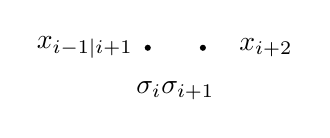
\begin{tikzpicture}[x=1cm,y=1cm]
\node at (0,0) {$x_{\unsure{i-1|i+1}}$};
\fill (0.8,0) circle (1.1pt); \fill (1.5,0) circle (1.1pt);
\node at (2.3,0) {$x_{i+2}$};
\node at (1.15,-.55) {$\sigma_i\sigma_{i+1}$};
\end{tikzpicture}}
\[
\sigma_0\sigma_1,\sigma_1\sigma_2,\ldots,\sigma_{n-2}\sigma_{n-1}
\]
\[
N=\prod_1^{n-1}s_i=\prod_1^{n-1}s'_i=\operatorname{card}G
\qquad G\ni\sigma_0,\ldots,\sigma_{n-1}
\]
\[
\left\{\begin{aligned}
s'_if_{i+1}&=f_is_{i+1}\qquad(0\leq i\leq n-1)\\
s&
\end{aligned}\right.
\qquad
\frac{f_i}{s'_i}=\frac{f_{i+1}}{\unsure{f_{i+1}|s_{i+1}}}=\unsure{f|\delta}
\]

\figure{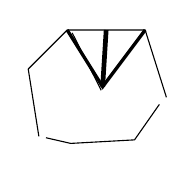
\begin{tikzpicture}[scale=.9]
\draw (0,.65)--(.55,1.2)--(1.65,1.2)--(1.95,.25);
\draw (1.85,.15)--(1.5,-.35)--(.6,-.4)--(.25,-.32);
\draw (.15,-.3)--(0,.65);
\draw[line width=1.2pt] (.55,1.2)--(1.05,.4)--(1.65,1.2);
\draw[line width=1.7pt] (1.05,.4)--(1.1,1.2);
\draw (.62,1.16)--(1.03,.35);
\end{tikzpicture}}

\figure{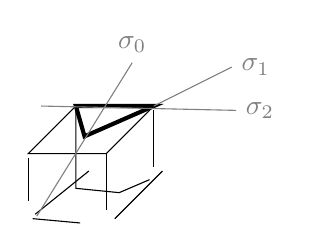
\begin{tikzpicture}[scale=1.1]
\draw (0,1)--(.55,1.55)--(1.45,1.55)--(.9,1)--cycle;
\draw (0,.95)--(0,.45) (.9,1)--(.9,.35) (1.45,1.5)--(1.45,.85);
\draw (.55,1.5)--(.55,.6)--(1.05,.55)--(1.4,.7);
\draw (.05,.25)--(.6,.2) (1,.25)--(1.55,.8);
\draw (.08,.3)--(.7,.8);
\draw[line width=1.5pt] (.55,1.55)--(1.45,1.55)--(.65,1.2)--cycle;
\draw[gray] (.1,.28)--(1.2,2.05) node[above] {$\sigma_0$};
\draw[gray] (1.45,1.55)--(2.35,2) node[right] {$\sigma_1$};
\draw[gray] (.15,1.55)--(2.4,1.5) node[right] {$\sigma_2$};
\end{tikzpicture}}

\figure{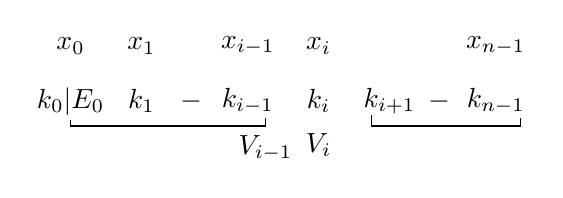
\begin{tikzpicture}[x=.9cm,y=.7cm]
\node at (0,1) {$x_0$}; \node at (1,1) {$x_1$};
\node at (2.5,1) {$x_{i-1}$}; \node at (3.5,1) {$x_i$};
\node at (6,1) {$x_{n-1}$};
\node at (0,0) {$\unsure{k_0|E_0}$}; \node at (1,0) {$k_1$};
\node at (1.7,0) {$-$}; \node at (2.5,0) {$k_{i-1}$};
\node at (3.5,0) {$k_i$}; \node at (4.5,0) {$k_{i+1}$};
\node at (5.2,0) {$-$}; \node at (6,0) {$k_{n-1}$};
\draw (0,-.35)--(0,-.45)--(2.75,-.45)--(2.75,-.3);
\node at (2.75,-.85) {$V_{i-1}$}; \node at (3.5,-.8) {$V_i$};
\draw (4.25,-.25)--(4.25,-.45)--(6.35,-.45)--(6.35,-.3);
\end{tikzpicture}}

\figure{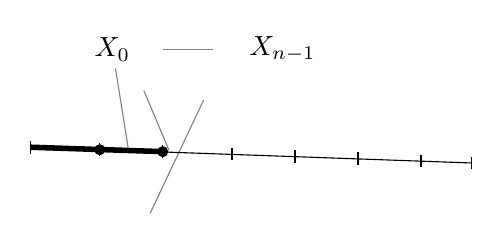
\begin{tikzpicture}[x=.8cm,y=.8cm]
\node at (1.3,1.7) {$X_0$}; \draw[gray] (2.1,1.7)--(2.9,1.7);
\node at (4,1.7) {$X_{n-1}$};
\draw[gray] (1.35,1.4)--(1.55,.15) (1.8,1.05)--(2.2,.1) (2.75,.9)--(1.9,-.9);
\draw (0,.15)--(7,-.1); \draw[line width=2pt] (0,.15)--(2.1,.08);
\foreach \x/\y in {0/.15,1.1/.11,2.1/.08,3.2/.04,4.2/.0,5.2/-.03,6.2/-.07,7/-.1}{\draw (\x,\y+.10)--(\x,\y-.10);}
\fill (1.1,.11) circle (2pt); \fill (2.1,.08) circle (2pt);
\end{tikzpicture}}
% archive sheet number: 123

\scanpage{125}
% The supplied scan is upside down; text transcribed in its reading orientation.
% letterhead
UNIVERSITÉ DES SCIENCES ET TECHNIQUES\\
DU LANGUEDOC\\
Place Eugène Bataillon\\
34060 MONTPELLIER CEDEX\\
\makebox[6cm]{\rule{1cm}{0.4pt}}\\
Tél. : 63.91.44 -- Télex : USTMONT 49944 F\\

ACADÉMIE DE MONTPELLIER\\
\makebox[7cm]{\rule{1.8cm}{0.4pt}}

Montpellier, le \quad 17 JUIN 1976 \quad 19\\

Le Secrétaire Général\\
à\\
Monsieur le Professeur \handwritten{Grothendieck}\\
Membre du Jury du Concours IPES\\
% printed form: dotted leader continues under handwritten subject.
\makebox[0pt][l]{\makebox[7cm]{\dotfill}}\hspace*{1.7cm}\handwritten{Math\unsure{è|é}matiques}

Monsieur le Professeur,\\

En l'absence de Monsieur MAURIN, j'ai l'honneur de vous communiquer ci-dessous la date de la délibération en vue de l'admissibilité au Concours IPES 1976 :

1) \uline{Concours IPES MATHEMATIQUES} :

Délibération le vendredi 2 Juillet à 14 H 30 salle de commissions N° 2 - Bâtiment administratif -

2) \uline{Concours IPES SCIENCES PHYSIQUES} :

Délibération le vendredi 2 Juillet à 9 H - salle de commissions n° 2 Bâtiment administratif.

Veuillez agréer, Monsieur le Professeur, l'expression de mes\\
sentiments distingués.\\

P. le Secrétaire Général,\\
\handwritten{\unsure{J. Doukhan|Doukhan}}\\
\uline{M. DOUKHAN.}
% stamp: ACADÉMIE DE MONTPELLIER; UNIVERSITÉ DES SCIENCES et TECHNIQUES DU LANGUEDOC; star
% archive sheet number: 124
